\setcounter{page}{3}
\chapter{Теоретическая часть}
\section{Базис языка Lisp.}
Базис~---~это минимальный набор правил/конструкций языка, к которым могут быть сведены все остальные. Базис языка Lisp представлен атомами, структурами, базовыми функциями, базовыми функционалами. Некоторые базисные функции: $car$, $cdr$, $cons$, $list$, $lambda$, $quote$, $eq$, $eql$, $equal$, $eval$, $apply$, $funcall$.

\section{Классификация функций языка Lisp.}
Среди функций в языке Lisp выделяют бызисные, пользовательские и функции ядра. Также, по реализации функции можно разделить на:
\begin{itemize}
	\item чистые (не создающие побочных эффектов, принимающие фиксированное число аргументов, не получающие данные неявно, результат работы которых не зависит от внешних переменных);
	\item особые, или формы;
	\item функции более высоких порядков, или функционалы (функции, результатом и/или аргументом которых является функция).
\end{itemize}

\section{Способы создания функций в языке Lisp.}
Функцию можно определить двумя способами: неименованную с помощью $lambda$ и именованную с помощью $defun$.

\begin{equation}
	\nonumber (lambda \quad (x_1 \quad x_2 \quad ... \quad x_n) \quad f),
\end{equation}
где $f$~---~тело функции, $x_i, i = \overline{1, n}$~---~формальные параметры.

\begin{equation}
	\nonumber (defun \quad <\text{имя}> \quad [lambda] \quad (x_1 \quad x_2 \quad ... \quad x_n) \quad f),
\end{equation}
где $f$~---~тело функции, $x_i, i = \overline{1, n}$~---~формальные параметры. Тогда имя будет ссылкой на описание функции.

\section{Функции $car$, $cdr$, $eq$, $eql$, $equal$, $equalp$.}
Функции $car$, $cdr$ являются базовыми функциями доступа к данным.

$car$ принимает точечную пару или список в качестве аргумента и возвращает указатель на первый элемент (если список пустой, то $Nil$). $cdr$ принимает точечную пару или список в качестве аргумента и возвращает все элементы, кроме первого или $Nil$ (указатель на хвост списка).

Функции сравнения~---~$eq$, $eql$, $equal$, $equalp$.

$eq$ возвращает истину тогда и только тогда, когда ее аргументы соответствуют одному и тому же объекту в памяти. $eql$ возвращает истину, если его аргументы равны с точки зрения $eq$, или если это числа одинакового типа и с одинаковыми значениями, или если это одинаковые буквы. $equal$ возвращает истину, если его аргументы равны с точки зрения $eql$,  либо являются списковыми ячейками, чьи $car$ и $cdr$ эквивалентны с точки зрения $equal$, либо являются строками (два объекта равны тогда и только тогда, когда их печатные представления одинаковы). $equalp$ возвращает истину, если его аргументы равны с точки зрения $equal$,  либо являются списковыми ячейками, чьи $car$ и $cdr$ эквивалентны с точки зрения $equalp$, либо являются списками одинаковой длины, элементы которых эквивалентны с точки зрения $equalp$; если они являются символами и удовлетворяют условию char-equal, которое игнорирует алфавитный регистр и некоторые другие атрибуты символов; если они являются числами и имеют одинаковое числовое значение, даже если они относятся к разным типам.

\section{Назначение и отличие в работе $cons$ и $list$.}
Функции $list$, $cons$ являются функциями создания списков ($cons$~---~базисная, $list$~---~нет). 

$cons$ принимает 2 аргумента (1-ый необязательно список, 2-ой список), создает списковую ячейку и устанавливает два указателя на аргументы. Если 2-ой аргумент $cons$~---~атом, то формируется точечная пара.

$list$ принимает переменное число аргументов, создаёт списковые ячейки, количество которых соответствует количеству переданных параметров, и расставляет указатели. Возвращает список, элементы которого~---~переданные в функцию аргументы.

Отличия:
\begin{itemize}
	\item количество аргументов (у $cons$~---~фиксированное (2), у $list$~---~переменное);
	\item результат (у $cons$~---~бинарный узел, у $list$~---~список);
	\item реализация в памяти.
\end{itemize}

\newpage

\chapter{Практическая часть}
\section{Задание №1}
Составить диаграмму вычисления следующих выражений:
\begin{enumerate}
	\item $(equal \quad 3 \quad (abs -3))$;
	\item $(equal \quad (+ \quad 1 \quad 2) \quad 3)$;
	\item $(equal \quad (* \quad 4 \quad 7) \quad 21)$;
	\item $(equal \quad (* \quad 2 \quad 3) \quad (+ \quad 7 \quad 2))$;
	\item $(equal \quad (- \quad 7 \quad 3) \quad (* \quad 3 \quad 2))$;
	\item $(equal \quad (abs \quad (- \quad 2 \quad 4)) \quad 3))$.
\end{enumerate}

Диаграммы приведены на рисунках ниже.

\begin{table}[h!]
  \centering
  \begin{tabular}{p{1\linewidth}}
    \centering
    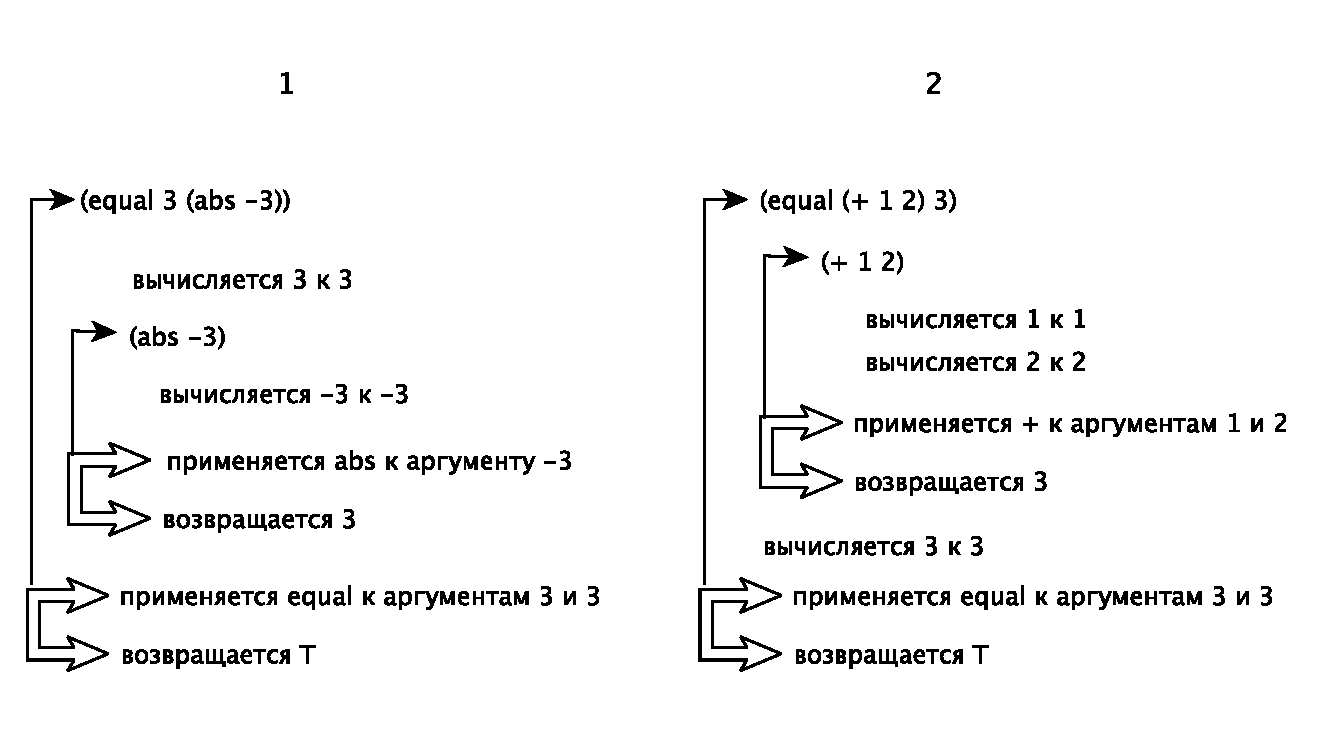
\includegraphics[width=1\linewidth]{./images/1&2.pdf}
    \captionof{figure}{Примеры №1 и №2}
    \label{img:1}
  \end{tabular}
\end{table}

\begin{table}[h!]
  \centering
  \begin{tabular}{p{1\linewidth}}
    \centering
    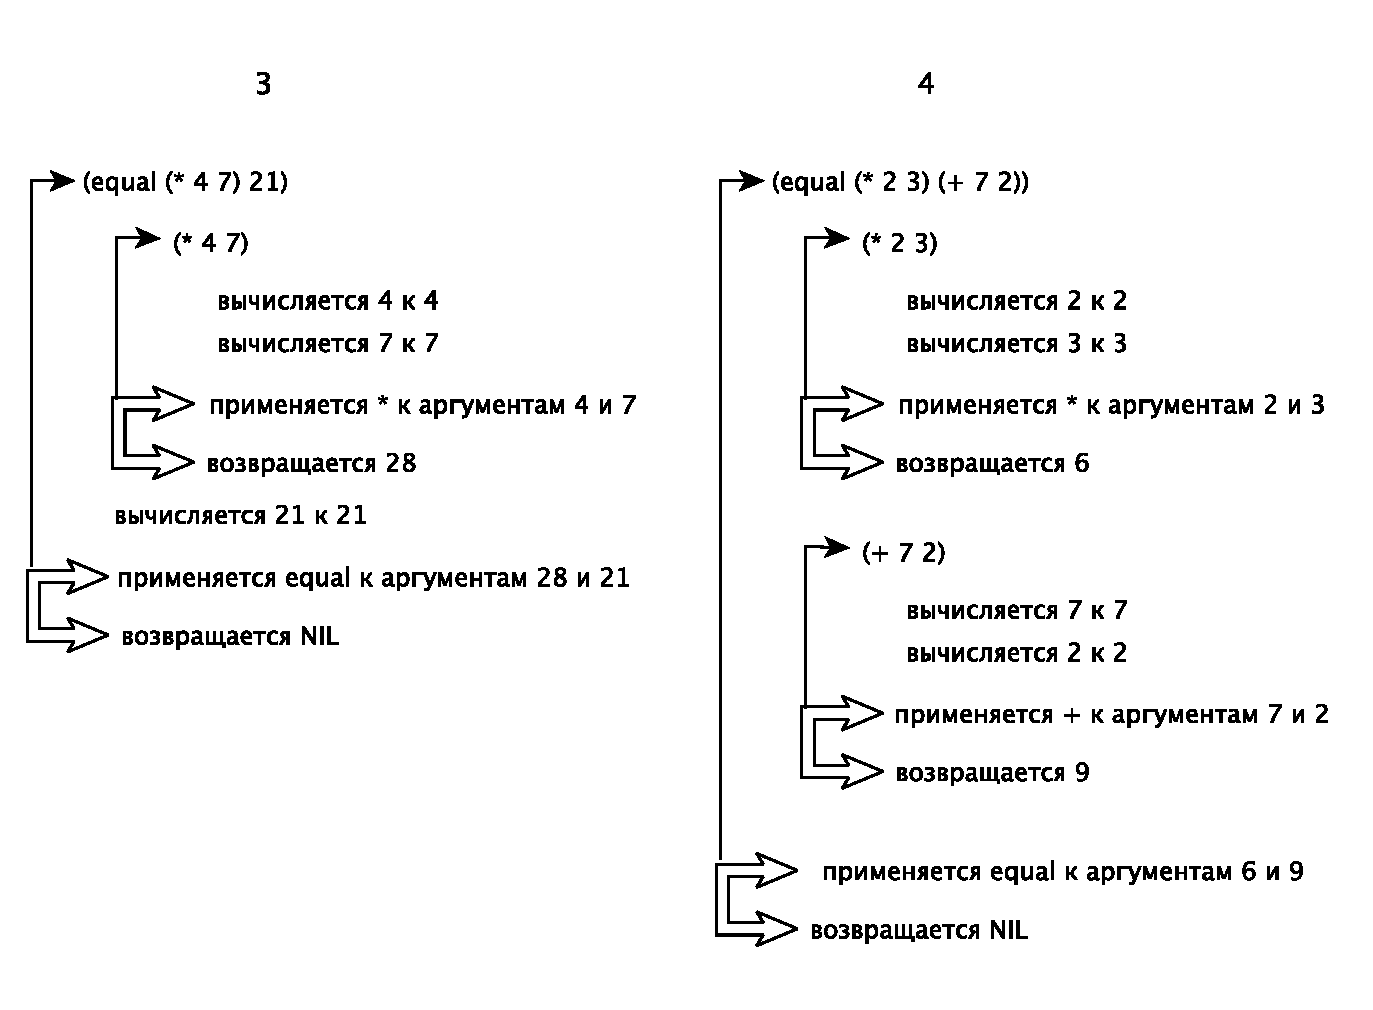
\includegraphics[width=0.8\linewidth]{./images/3&4.pdf}
    \captionof{figure}{Примеры №3 и №4}
    \label{img:1}
  \end{tabular}
\end{table}

\begin{table}[h!]
  \centering
  \begin{tabular}{p{1\linewidth}}
    \centering
    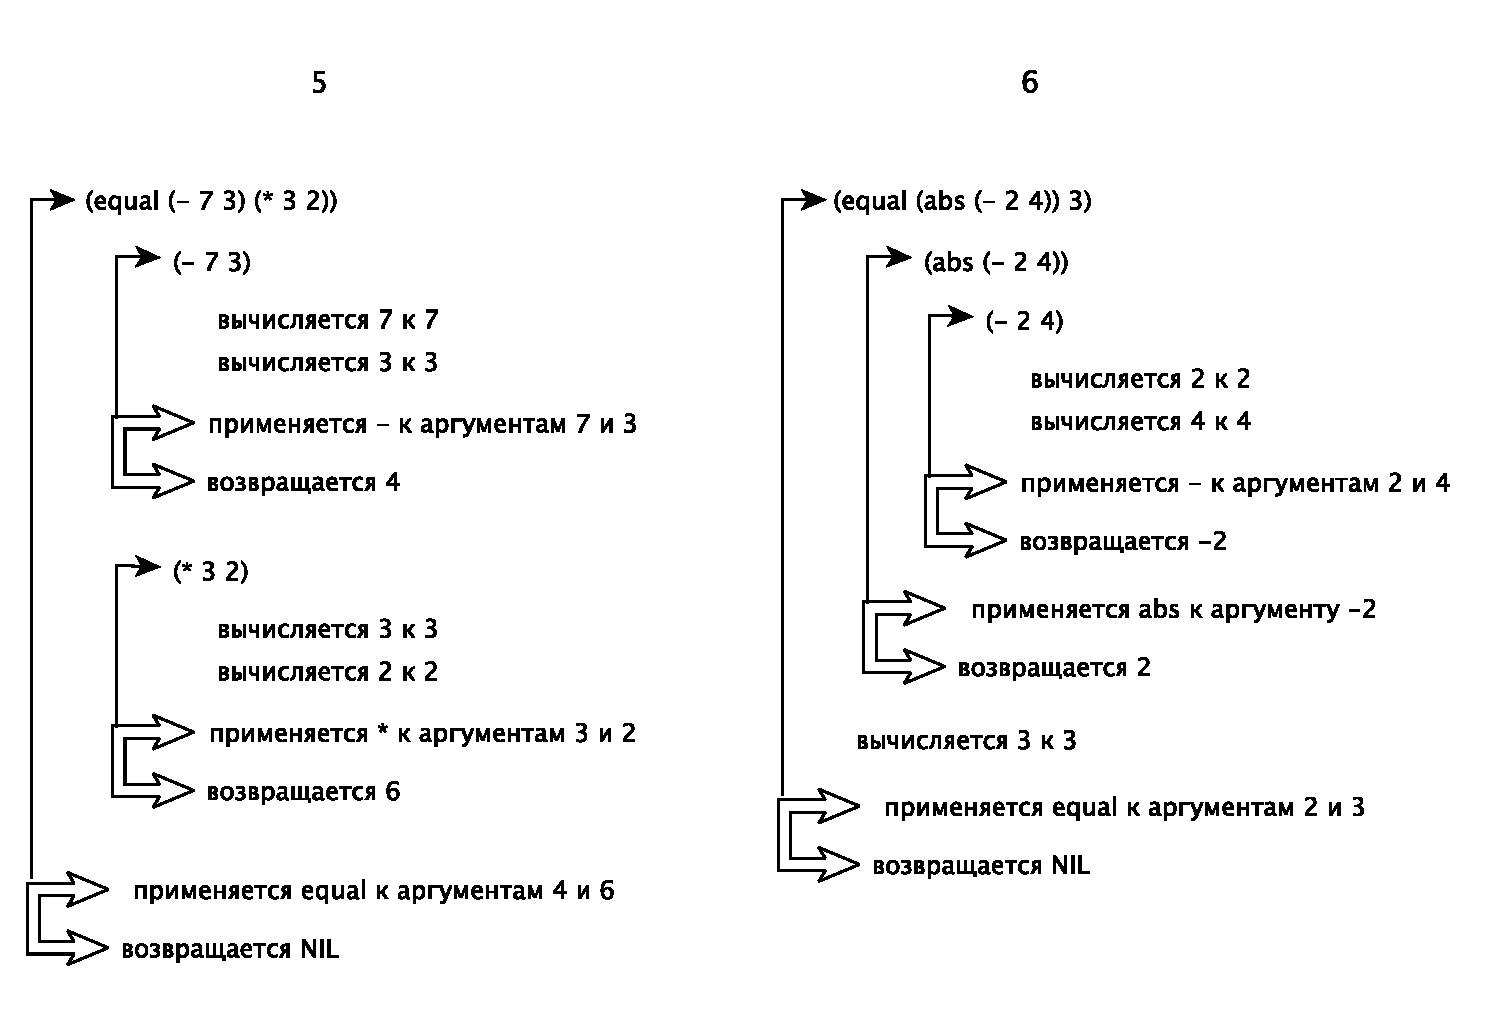
\includegraphics[width=0.8\linewidth]{./images/5&6.pdf}
    \captionof{figure}{Примеры №5 и №6}
    \label{img:1}
  \end{tabular}
\end{table}

\section{Задание №2}
Написать функцию, вычисляющую гипотенузу прямоугольного треугольника по заданным катетам и составить диаграмму её вычисления.

\begin{code}
\caption{Задание №2}
\label{code:bf2}
\begin{minted}{lisp}
(defun get_hypot (k1 k2) (sqrt (+ (* k1 k1) (* k2 k2))))
(get_hypot 4 3)
\end{minted}
\end{code}

Диаграмма вычисления для $get\text{\_}hypot$ представлена ниже.

\begin{table}[h!]
  \centering
  \begin{tabular}{p{1\linewidth}}
    \centering
    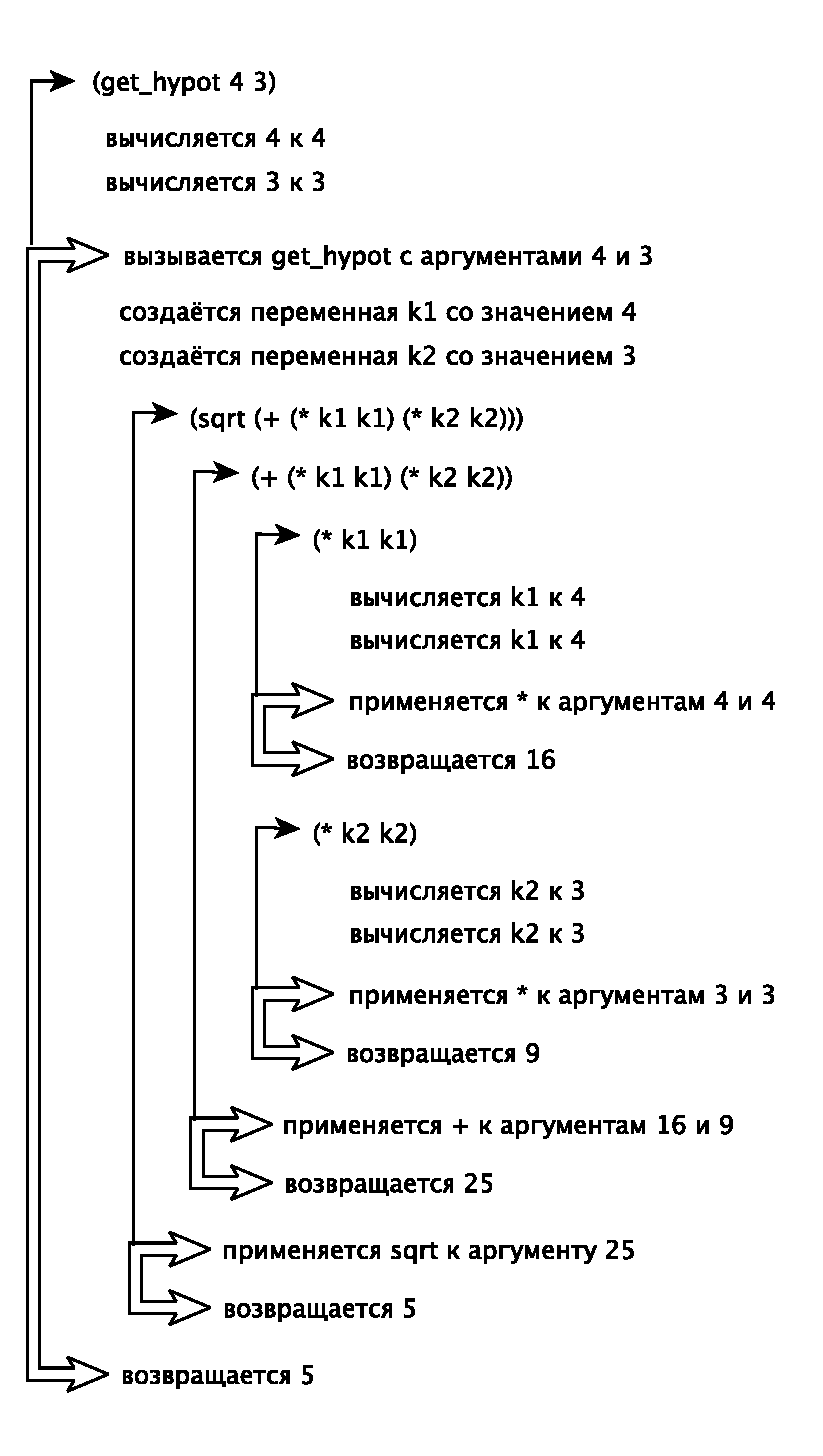
\includegraphics[width=0.5\linewidth]{./images/2-1.pdf}
    \captionof{figure}{Диаграмма вычислений для $get\text{\_}hypot$}
    \label{img:1}
  \end{tabular}
\end{table}

\section{Задание №3}
Каковы результаты вычисления следующих выражений? (объяснить возможную ошибку и варианты ее устранения).

\begin{code}
\caption{Задание №3}
\label{code:bf3}
\begin{minted}{lisp}
(list 'a c)
; *** - SYSTEM::READ-EVAL-PRINT: variable C has no value
; "с" воспринимается не как данное, а как имя переменной
(list 'a 'c)
; (A C)
(setf c 3)
; 3
(list 'a c)
; (A 3)

(cons 'a (b c))
; *** - EVAL: undefined function B
; первая часть выражения в скобках по умолчанию воспринимается как
; действие (функция)
(cons 'a '(b c))
; (A B C)

(caddr (1 2 3 4 5))
; *** - EVAL: 1 is not a function name; try using a symbol instead
; первая часть выражения в скобках по умолчанию воспринимается как
; действие (функция)
(caddr '(1 2 3 4 5))
; 3
\end{minted}
\end{code}

\newpage

\begin{code}
\caption{Задание №3}
\label{code:bf4}
\begin{minted}{lisp}
(cons 'a 'b 'c)
; *** - EVAL: too many arguments given to CONS: (CONS 'A 'B 'C)
; это функция с фиксированным числом аргументов (2)
(cons 'a '(b c))
; (A B C)
(cons '(a b) 'c)
; ((A B) . C)

(list 'a (b c))
; *** - EVAL: undefined function B
; первая часть выражения в скобках по умолчанию воспринимается как
; действие (функция)
(list 'a '(b c))
; (A (B C))
(list 'a 'b 'c)
; (A B C)

(list a '(b c))
; *** - SYSTEM::READ-EVAL-PRINT: variable A has no value
; "а" воспринимается не как данное, а как имя переменной
(list 'a '(b c))
; (A (B C))
(setf a 2)
; 2
(list a '(b c))
; (2 (B C))

(list (+ 1 '(length '(1 2 3))))
; *** - +: (LENGTH '(1 2 3)) is not a number
; применение символа апострофа означает блокировку вычислений, то есть 
; "length" воспринимается как строковое данное, а не как функция
(list (+ 1 (length '(1 2 3))))
; (4)
\end{minted}
\end{code}

\newpage

\section{Задание №4}
Написать функцию $longer \text{\_} than$ от двух списков-аргументов, которая возвращает $Т$, если первый аргумент имеет большую длину.

\begin{code}
\caption{Задание №4}
\label{code:bf4}
\begin{minted}{lisp}
(defun longer_than (l1 l2) (> (length l1) (length l2)))
(longer_then (list 1 2 3) (list 1 2))
; T
Break 10 [13]> (longer_then (list 1 2) (list 1 2))
; NIL
\end{minted}
\end{code}

\section{Задание №5}
Каковы результаты вычисления следующих выражений?
\begin{enumerate}
	\item $(cons \quad 3 \quad (list \quad 5 \quad 6))$;
	\item $(cons \quad 3 \quad '(list \quad 5 \quad 6))$;
	\item $(list \quad 3 \quad 'from \quad 9 \quad 'lives \quad (- \quad 9 \quad 3))$;
	\item $(+ \quad (length \quad for \quad 2 \quad too)) \quad (car \quad '(21 \quad 22 \quad 23)))$;
	\item $(cdr \quad '(cons \quad is \quad short \quad for \quad ans))$;
	\item $(car \quad (list \quad one \quad two))$.
\end{enumerate}

\begin{code}
\caption{Задание №5}
\label{code:bf5}
\begin{minted}{lisp}
(cons 3 (list 5 6))
; (3 5 6)

(cons 3 '(list 5 6))
; (3 LIST 5 6)

(list 3 'from 9 'lives (- 9 3))
; (3 FROM 9 LIVES 6)
\end{minted}
\end{code}

\newpage

\begin{code}
\caption{Задание №5}
\label{code:bf5}
\begin{minted}{lisp}
(+ (length for 2 too)) (car '(21 22 23)))
; *** - SYSTEM::READ-EVAL-PRINT: variable FOR has no value
(+ (length '(for 2 too)) (car '(21 22 23)))
; 24

(cdr '(cons is short for ans))
; (IS SHORT FOR ANS)

(car (list one two))
; *** - SYSTEM::READ-EVAL-PRINT: variable ONE has no value
(car (list 'one 'two))
; ONE
\end{minted}
\end{code}

\section{Задание №6}
% почему аргумент это обязательно список?
Дана функция $(defun \quad mystery \quad (x) \quad (list \quad (second \quad x) \quad (first \quad x)))$. Какие результаты вычисления следующих выражений?
\begin{enumerate}
	\item $(mystery \quad (one \quad two))$;
	\item $(mystery \quad one \quad 'two))$;
	\item $(mystery \quad (last \quad one \quad two))$;
	\item $(mystery \quad free)$.
\end{enumerate}

\begin{code}
\caption{Задание №6}
\label{code:bf4}
\begin{minted}{lisp}
(mystery (one two))
; *** - EVAL: undefined function ONE
(mystery '(one two))
; (TWO ONE)
\end{minted}
\end{code}

\newpage

\begin{code}
\caption{Задание №6}
\label{code:bf4}
\begin{minted}{lisp}
(mystery one 'two))
; *** - SYSTEM::READ-EVAL-PRINT: variable ONE has no value
(mystery '(one two))
; (TWO ONE)

(mystery (last one two))
; *** - SYSTEM::READ-EVAL-PRINT: variable ONE has no value
(mystery (last '(one two)))
; (NIL TWO)

(mystery free)
; *** - SYSTEM::READ-EVAL-PRINT: variable FREE has no value
(mystery '(free))
; (NIL FREE)
\end{minted}
\end{code}

\section{Задание №7}
Написать функцию, которая переводит температуру в системе Фаренгейта температуру по Цельсию $(defun \quad f-to-c \quad (temp)...)$.

Формулы: $c = \frac{5}{9} \cdot (f - 320)$; $f = \frac{9}{5} \cdot c + 32.0$.

Как бы назывался роман Р.Брэдбери "+451 по Фаренгейту" в системе по Цельсию?

\begin{code}
\caption{Задание №7}
\label{code:bf4}
\begin{minted}{lisp}
(defun f_to_c (temp) (* (/ 5 9) (- temp 320)))
(defun c-to-f (temp) (+ (* (/ 9 5) temp) 32.0))

(f_to_c 451)
; 655/9 ~ 73
\end{minted}
\end{code}

\newpage

\section{Задание №8}
Что получится при вычисления каждого из выражений?
\begin{enumerate}
	\item $(list \quad 'cons \quad t \quad NIL)$;
	\item $(eval \quad (eval \quad (list \quad 'cons \quad t \quad NIL)))$;
	\item $(apply \quad \#cons \quad "(t \quad NIL))$;
	\item $(list \quad 'eval \quad NIL)$;
	\item $(eval \quad (list \quad 'cons \quad t \quad NIL))$;
	\item $(eval \quad NIL)$;
	\item $(eval \quad (list \quad 'eval \quad NIL))$.
\end{enumerate}

\begin{code}
\caption{Задание №8}
\label{code:bf4}
\begin{minted}{lisp}
(list 'cons t NIL)
; (CONS T NIL)

(eval (list 'cons t NIL))
; (T)

(eval (eval (list 'cons t NIL)))
; *** - EVAL: undefined function T

(apply #cons "(t NIL))
; *** - READ from #<INPUT CONCATENATED-STREAM #<INPUT STRING-INPUT-STREAM> 
; #<IO TERMINAL-STREAM>>: bad syntax for complex number: #CONS
(apply #'cons '(t NIL))
; (T)

(eval NIL)
; NIL
\end{minted}
\end{code}

\newpage

\begin{code}
\caption{Задание №8}
\label{code:bf4}
\begin{minted}{lisp}
(list 'eval NIL)
; (EVAL NIL)

(eval (list 'eval NIL))
; NIL
\end{minted}
\end{code}

\newpage